\chapter{Co-expression of NER repair factors}
The previously described model-aided analysis of the DNA repair process revealed the link between the emergent phenomenon of rapidly exchanging and transiently interacting NER components with the experimentally observed slow first-order kinetics of repair. An important functional consequence of this kinetic design is that the control of the repair rate is shared by all repair factors. This manifests in the mathematical prediction of uniformly distributed response coefficients, which quantify the relative change of the repair rate in answer to changes in the nuclear repair protein concentration. Exploiting the natural variability in NER factor expression, their moderate control on the rate of repair could be experimentally resolved for different repair phases. These findings, however, were made under the assumption of a functional independence of the individual NER components. Effects resulting from co-regulated NER factor expression or protein degradation were so far neglected as a first approximation.  \\
To test this assumption, in the following chapter we will investigate a potential cross-correlation among the involved repair factors experimentally. Surprisingly, we find that the nuclear expression of five pairwise measured repair factors (XPC, TFIIH, XPA, XPF and RPA) is indeed strong positively correlated, whereas there is no correlation with the repair-independent cell cycle marker \textbf{Ki67}. This result suggests an additional control mechanism orchestrating NER factor expression on the transcriptional or translational level.    

- sentence about who did what

\section{Co-staining experiments}

Using fluorescence microscopy for the quantitative analysis of the NER process proved to result in accurate measurements of the nuclear expression and UV-induced repair dynamics of the individual repair factors at a high signal to noise ratio. This applies for the stably transfected fluorescently tagged repair protein expression as well as for an immunocytochemistry approach with an indirect antibody-labeling of the measured NER factors. The latter technique has the advantage that once a specifically binding antibody is established it can be applied on all cell types containing the desired antigen. On this basis, indirect labeling of the primary antibody with a secondary antibody allows for the combinatorial tagging of multiple antigens restricted only by cross-reactions between antibodies originating from the same host species \cite{Burry2011,Giepmans2006}. Following such a protocol we established five single cell double stainings (cf.\ Table \ref{tab:co-staining} using the primary and secondary antibodies listed in Table \textbf{tbm}. 


\begin{table}[h!]
	\centering
	\begin{tabular}{cccccc}
		\hline
			\rule{0pt}{2ex}
			&\textbf{XPC} & \textbf{TFIIH} & \textbf{XPA} & \textbf{XPF} & \textbf{RPA}\\ \hline
			\rule{0pt}{3ex}
\textbf{XPC}&        X    &           X    & X            &         X    & X            \\ \hline
			\rule{0pt}{3ex}
\textbf{TFIIH}&           & -              & -            & X            & -             \\ \hline
			\rule{0pt}{3ex}
\textbf{XPA}&             &                & -            & X            & X             \\ \hline
			\rule{0pt}{3ex}
\textbf{XPF}&             &                &              & -            & -              \\ \hline
			\rule{0pt}{3ex}
\textbf{RPA}&             &                &              &              & -               \\ \hline
			\rule{0pt}{3ex}
		
	\end{tabular}
	\caption{\textbf{Mean and standard deviation of the variability in nuclear XPC, TFIIH, XPA and XPF expression.} }\label{tab:co-staining}
\end{table}   

Additional two measurements were possible using a directly labeled monoclonal mouse XPC-antibody after an initial indirect labeling step of one of the other four repair factors. The combined measurement of XPC ...    




microscopy analysis was extended

- Dapi for the segmentation of the nucleus
- microscopy was done with Leica widefield 
- 3D imaging


\begin{figure}[htbp]
	\begin{center}
		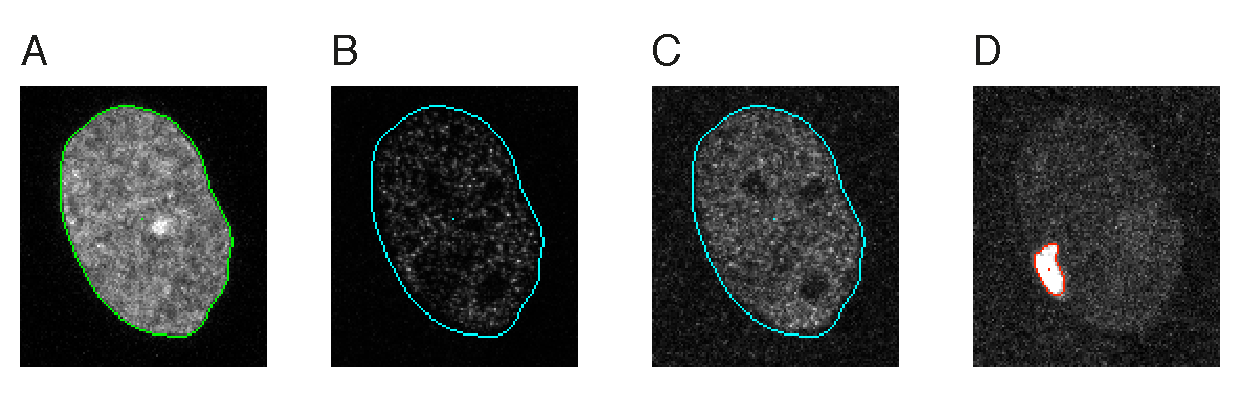
\includegraphics[width=1\textwidth]{Abbildungen/figure4_1.pdf}
		\caption{\textbf{Blubb.} A) B) }
		\label{fig:coStaining}
	\end{center}
\end{figure}

\subsection{Nuclear expression of NER factors is strongly correlated}

\begin{figure}[htbp]
	\begin{center}
		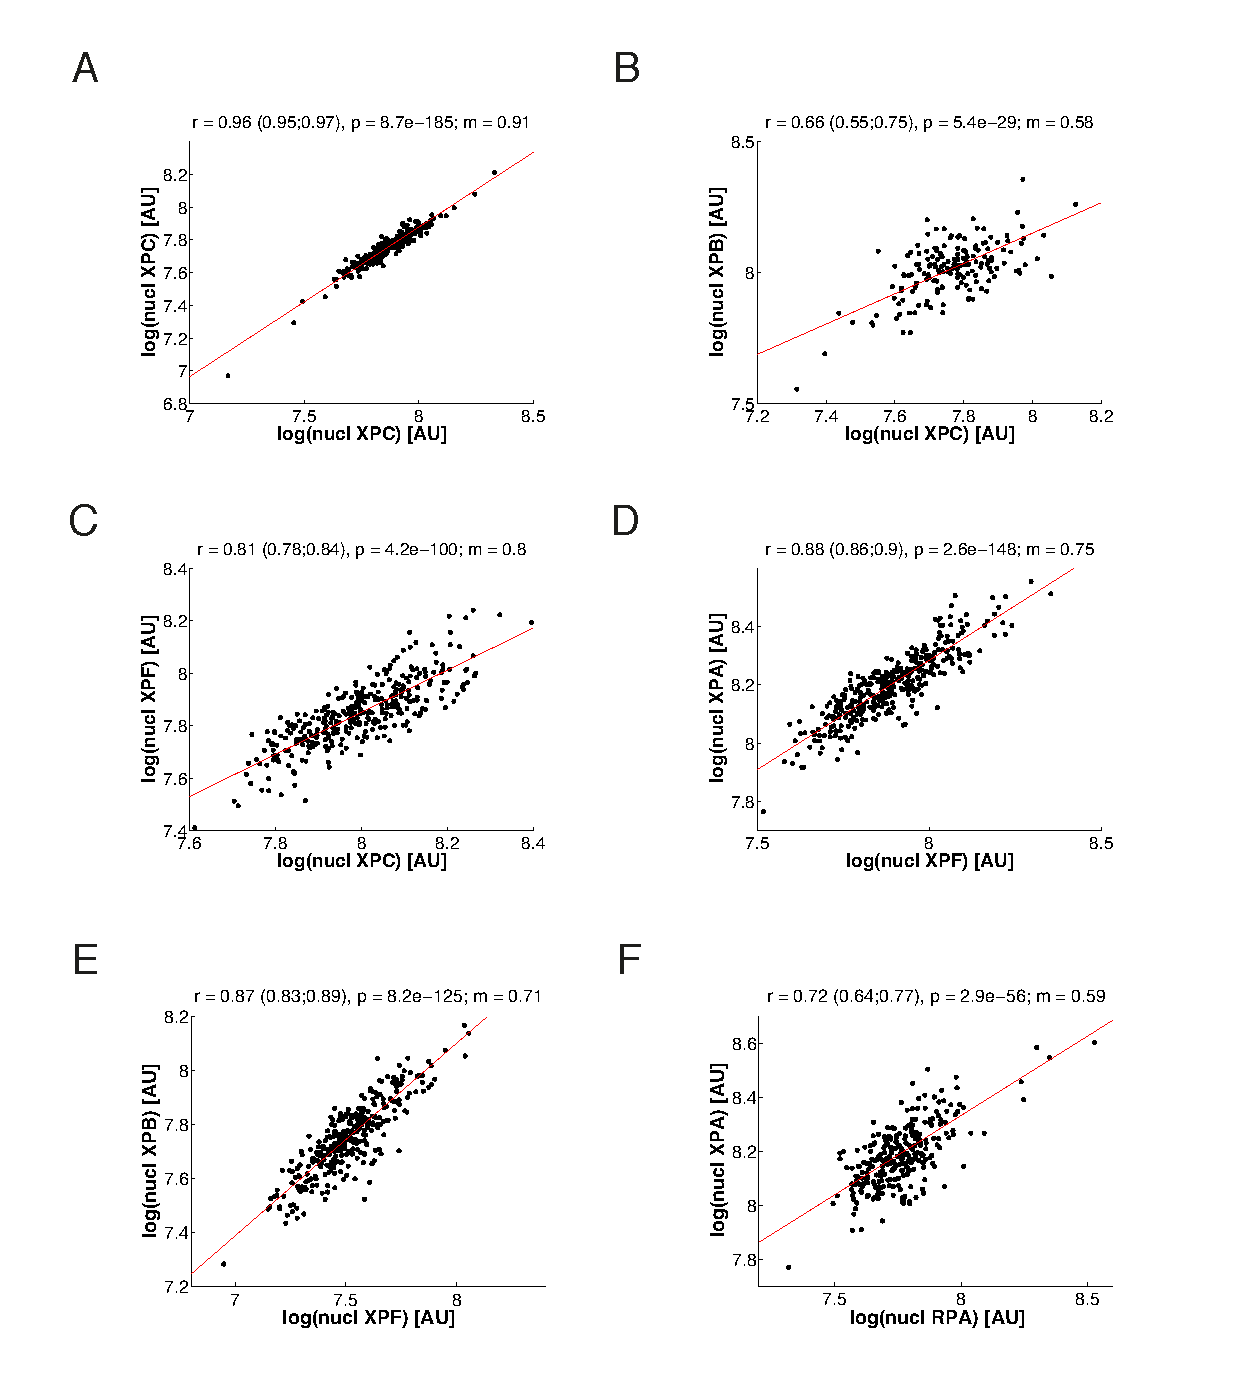
\includegraphics[width=1\textwidth]{Abbildungen/figure4_2.pdf}
		\caption{\textbf{Blubb.} A) B) }
		\label{fig:coExpressionData}
	\end{center}
\end{figure}


\begin{figure}[htbp]
	\begin{center}
		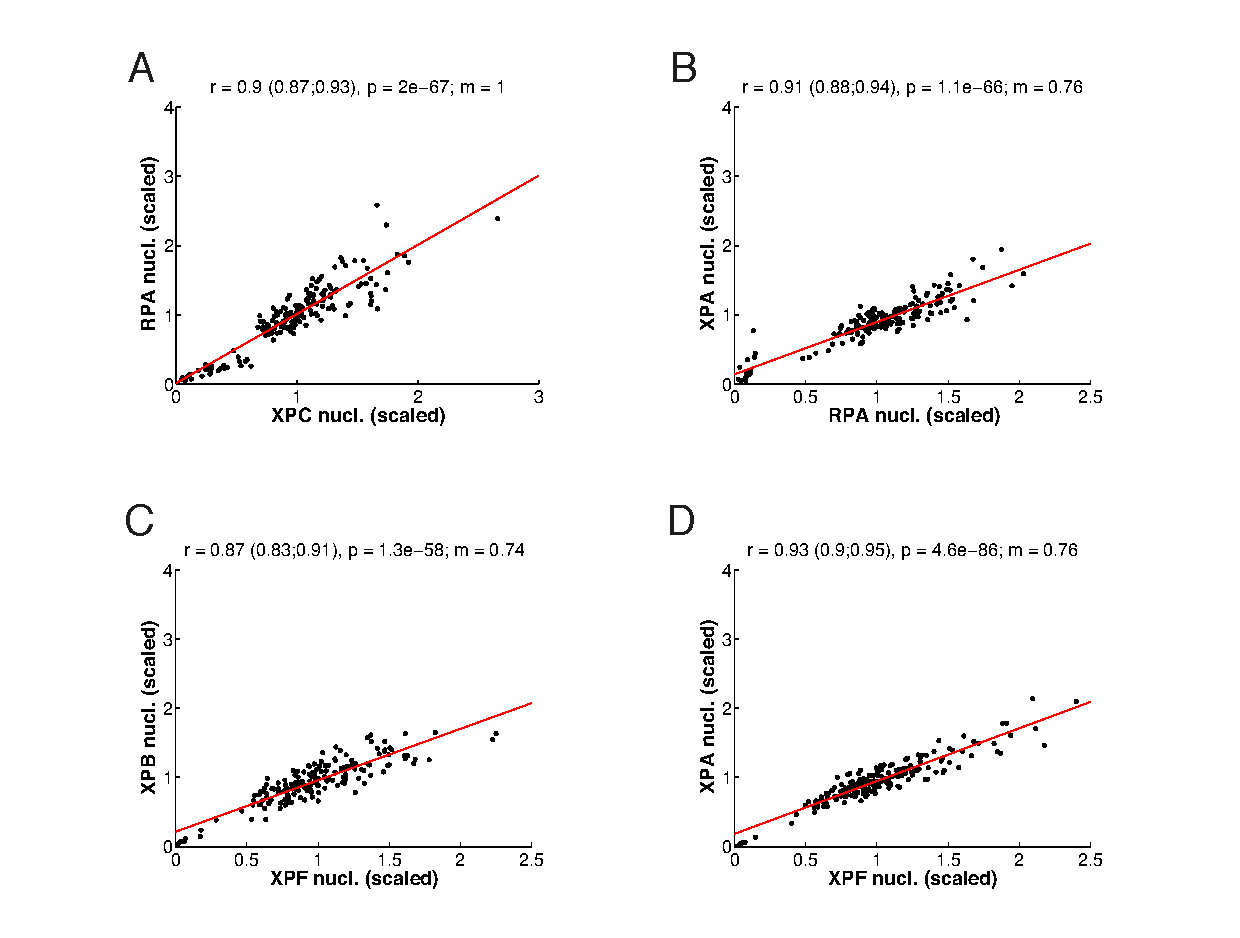
\includegraphics[width=1\textwidth]{Abbildungen/figure4_3.pdf}
		\caption{\textbf{Blubb.} A) B) }
		\label{fig:coExpressionData_woDamage}
	\end{center}
\end{figure}

\subsection{Flow cytometry verification}

